% Options for packages loaded elsewhere
\PassOptionsToPackage{unicode}{hyperref}
\PassOptionsToPackage{hyphens}{url}
\PassOptionsToPackage{dvipsnames,svgnames,x11names}{xcolor}
%
\documentclass[
  letterpaper,
  DIV=11,
  numbers=noendperiod]{scrartcl}

\usepackage{amsmath,amssymb}
\usepackage{iftex}
\ifPDFTeX
  \usepackage[T1]{fontenc}
  \usepackage[utf8]{inputenc}
  \usepackage{textcomp} % provide euro and other symbols
\else % if luatex or xetex
  \usepackage{unicode-math}
  \defaultfontfeatures{Scale=MatchLowercase}
  \defaultfontfeatures[\rmfamily]{Ligatures=TeX,Scale=1}
\fi
\usepackage{lmodern}
\ifPDFTeX\else  
    % xetex/luatex font selection
\fi
% Use upquote if available, for straight quotes in verbatim environments
\IfFileExists{upquote.sty}{\usepackage{upquote}}{}
\IfFileExists{microtype.sty}{% use microtype if available
  \usepackage[]{microtype}
  \UseMicrotypeSet[protrusion]{basicmath} % disable protrusion for tt fonts
}{}
\makeatletter
\@ifundefined{KOMAClassName}{% if non-KOMA class
  \IfFileExists{parskip.sty}{%
    \usepackage{parskip}
  }{% else
    \setlength{\parindent}{0pt}
    \setlength{\parskip}{6pt plus 2pt minus 1pt}}
}{% if KOMA class
  \KOMAoptions{parskip=half}}
\makeatother
\usepackage{xcolor}
\setlength{\emergencystretch}{3em} % prevent overfull lines
\setcounter{secnumdepth}{5}
% Make \paragraph and \subparagraph free-standing
\ifx\paragraph\undefined\else
  \let\oldparagraph\paragraph
  \renewcommand{\paragraph}[1]{\oldparagraph{#1}\mbox{}}
\fi
\ifx\subparagraph\undefined\else
  \let\oldsubparagraph\subparagraph
  \renewcommand{\subparagraph}[1]{\oldsubparagraph{#1}\mbox{}}
\fi


\providecommand{\tightlist}{%
  \setlength{\itemsep}{0pt}\setlength{\parskip}{0pt}}\usepackage{longtable,booktabs,array}
\usepackage{calc} % for calculating minipage widths
% Correct order of tables after \paragraph or \subparagraph
\usepackage{etoolbox}
\makeatletter
\patchcmd\longtable{\par}{\if@noskipsec\mbox{}\fi\par}{}{}
\makeatother
% Allow footnotes in longtable head/foot
\IfFileExists{footnotehyper.sty}{\usepackage{footnotehyper}}{\usepackage{footnote}}
\makesavenoteenv{longtable}
\usepackage{graphicx}
\makeatletter
\def\maxwidth{\ifdim\Gin@nat@width>\linewidth\linewidth\else\Gin@nat@width\fi}
\def\maxheight{\ifdim\Gin@nat@height>\textheight\textheight\else\Gin@nat@height\fi}
\makeatother
% Scale images if necessary, so that they will not overflow the page
% margins by default, and it is still possible to overwrite the defaults
% using explicit options in \includegraphics[width, height, ...]{}
\setkeys{Gin}{width=\maxwidth,height=\maxheight,keepaspectratio}
% Set default figure placement to htbp
\makeatletter
\def\fps@figure{htbp}
\makeatother
\newlength{\cslhangindent}
\setlength{\cslhangindent}{1.5em}
\newlength{\csllabelwidth}
\setlength{\csllabelwidth}{3em}
\newlength{\cslentryspacingunit} % times entry-spacing
\setlength{\cslentryspacingunit}{\parskip}
\newenvironment{CSLReferences}[2] % #1 hanging-ident, #2 entry spacing
 {% don't indent paragraphs
  \setlength{\parindent}{0pt}
  % turn on hanging indent if param 1 is 1
  \ifodd #1
  \let\oldpar\par
  \def\par{\hangindent=\cslhangindent\oldpar}
  \fi
  % set entry spacing
  \setlength{\parskip}{#2\cslentryspacingunit}
 }%
 {}
\usepackage{calc}
\newcommand{\CSLBlock}[1]{#1\hfill\break}
\newcommand{\CSLLeftMargin}[1]{\parbox[t]{\csllabelwidth}{#1}}
\newcommand{\CSLRightInline}[1]{\parbox[t]{\linewidth - \csllabelwidth}{#1}\break}
\newcommand{\CSLIndent}[1]{\hspace{\cslhangindent}#1}

\usepackage{booktabs}
\usepackage{longtable}
\usepackage{array}
\usepackage{multirow}
\usepackage{wrapfig}
\usepackage{float}
\usepackage{colortbl}
\usepackage{pdflscape}
\usepackage{tabu}
\usepackage{threeparttable}
\usepackage{threeparttablex}
\usepackage[normalem]{ulem}
\usepackage{makecell}
\usepackage{xcolor}
\KOMAoption{captions}{tableheading}
\makeatletter
\makeatother
\makeatletter
\makeatother
\makeatletter
\@ifpackageloaded{caption}{}{\usepackage{caption}}
\AtBeginDocument{%
\ifdefined\contentsname
  \renewcommand*\contentsname{Table of contents}
\else
  \newcommand\contentsname{Table of contents}
\fi
\ifdefined\listfigurename
  \renewcommand*\listfigurename{List of Figures}
\else
  \newcommand\listfigurename{List of Figures}
\fi
\ifdefined\listtablename
  \renewcommand*\listtablename{List of Tables}
\else
  \newcommand\listtablename{List of Tables}
\fi
\ifdefined\figurename
  \renewcommand*\figurename{Figure}
\else
  \newcommand\figurename{Figure}
\fi
\ifdefined\tablename
  \renewcommand*\tablename{Table}
\else
  \newcommand\tablename{Table}
\fi
}
\@ifpackageloaded{float}{}{\usepackage{float}}
\floatstyle{ruled}
\@ifundefined{c@chapter}{\newfloat{codelisting}{h}{lop}}{\newfloat{codelisting}{h}{lop}[chapter]}
\floatname{codelisting}{Listing}
\newcommand*\listoflistings{\listof{codelisting}{List of Listings}}
\makeatother
\makeatletter
\@ifpackageloaded{caption}{}{\usepackage{caption}}
\@ifpackageloaded{subcaption}{}{\usepackage{subcaption}}
\makeatother
\makeatletter
\@ifpackageloaded{tcolorbox}{}{\usepackage[skins,breakable]{tcolorbox}}
\makeatother
\makeatletter
\@ifundefined{shadecolor}{\definecolor{shadecolor}{rgb}{.97, .97, .97}}
\makeatother
\makeatletter
\makeatother
\makeatletter
\makeatother
\ifLuaTeX
  \usepackage{selnolig}  % disable illegal ligatures
\fi
\IfFileExists{bookmark.sty}{\usepackage{bookmark}}{\usepackage{hyperref}}
\IfFileExists{xurl.sty}{\usepackage{xurl}}{} % add URL line breaks if available
\urlstyle{same} % disable monospaced font for URLs
\hypersetup{
  pdftitle={STA302 Final Project Proposal},
  pdfauthor={Ziqi Zhu; Author 2; Author 3},
  colorlinks=true,
  linkcolor={blue},
  filecolor={Maroon},
  citecolor={Blue},
  urlcolor={Blue},
  pdfcreator={LaTeX via pandoc}}

\title{STA302 Final Project Proposal\thanks{Code and data are available
at: https://github.com/zzq20010617/sta302Paper}}
\author{Ziqi Zhu \and Author 2 \and Author 3}
\date{October 23, 2024}

\begin{document}
\maketitle
\ifdefined\Shaded\renewenvironment{Shaded}{\begin{tcolorbox}[interior hidden, boxrule=0pt, sharp corners, frame hidden, breakable, enhanced, borderline west={3pt}{0pt}{shadecolor}]}{\end{tcolorbox}}\fi

\renewcommand*\contentsname{Table of contents}
{
\hypersetup{linkcolor=}
\setcounter{tocdepth}{3}
\tableofcontents
}
\hypertarget{introduction-350}{%
\section{Introduction (350)}\label{introduction-350}}

The gaming industry has experienced exponential growth in recent years,
with millions of players engaging in various games on platforms like
Steam. Understanding what influences average playtime in games is
crucial for game developers, publishers, and marketers. Average playtime
is a key indicator of player engagement and game success, and
investigating factors that impact it can provide valuable insights into
game design, pricing strategies, and marketing efforts. So our research
aims to explore the factors that influence the average playtime of games
available on Steam using a dataset we get from Kaggle. Specifically, we
will investigate how variables such as price, user ratings, and other
game characteristics contribute to player engagement, as measured by
playtime. From some previous papers, we learned that both positive and
negative reviews have a significant correlation with playtime, but the
effect is more pronounced for positive reviews(Brodschneider and Pirker
(2023)). Another paper found out that game pricing significantly affects
player engagement, with lower-priced games generally seeing higher
playtime.(Luisa et al. (2021)). The third paper did an empirical study
that also examined the influence of game reviews on playtime, focusing
on how the number and sentiment of reviews can affect player engagement.
It concludes that games with more positive reviews see increased
playtime, especially if those reviews highlight the game's quality(Lin
et al. (2019)). We found this problem suitable for linear regression
because it allows us to model the relationship between average playtime
(the dependent variable) and various predictors (price, ratings,
developer, etc.). This approach helps quantify how each factor
influences playtime, enabling a clear understanding of the impact of
different game attributes. By fitting a linear regression model, we can
determine which factors have statistically significant effects on
playtime, providing actionable insights for game developers and
marketers.

\hypertarget{data-description-300}{%
\section{Data description (300)}\label{data-description-300}}

We get the Steam games data(Davis (2023)) from Kaggle. The R programming
language (R Core Team (2023)) and packages readr(Wickham, Hester, and
Bryan (2024)), httr(Wickham (2023)), jsonlite(Ooms (2014)) were used to
download the data, dplyr(Wickham et al. (2023)) and lubridate(Grolemund
and Wickham (2011)) were used to clean the data. Data was originally
gathered from the Steam Store and SteamSpy APIs around May 2019. This
table Table~\ref{tbl-cle} shows the first 3 entries of cleaned data. We
are going to take average\_playtime as the response variable, it
measures the mean time (in minutes) that players spend on a game, a
summary of this variable is shown in Table~\ref{tbl-aveplaytime}. This
variable captures overall player engagement and serves as a good
indicator of how immerse or entertaining a game is. It is suitable for a
linear regression model because it is continuous and quantitative. The
predictors selected are price, positive ratings, negative ratings,
developer, and number of owners. All are numeric except for the number
of owners, which is categorical since it represents estimated ranges.
Price may influence playtime, as higher costs could lead to longer
engagement. Positive ratings and negative ratings are reviews of players
of that game and it can only be positive or negative. Positive ratings
likely correlate with greater playtime, while negative ratings could
indicate the opposite. Developer refers to the development company of
the game, which could affect playtime, with established studios often
producing longer, high-quality games. Lastly, the number of owners is an
estimated number of owners, containing lower and upper bounds (like
20000-50000), it could signal popularity, where more owners may suggest
higher average playtime. Summary of numerical predictors can be find in
table Table~\ref{tbl-predictor}.

\hypertarget{tbl-cle}{}
\begin{table}
\caption{\label{tbl-cle}Steam Games Data }\tabularnewline

\centering
\resizebox{\ifdim\width>\linewidth\linewidth\else\width\fi}{!}{
\begin{tabular}[t]{l|r|l|l|r|r|r|r|r|l|r}
\hline
release\_month & english & developer & publisher & achievements & positive\_ratings & negative\_ratings & average\_playtime & median\_playtime & owners & price\\
\hline
\cellcolor{gray!10}{Nov} & \cellcolor{gray!10}{1} & \cellcolor{gray!10}{Valve} & \cellcolor{gray!10}{Valve} & \cellcolor{gray!10}{0} & \cellcolor{gray!10}{124534} & \cellcolor{gray!10}{3339} & \cellcolor{gray!10}{17612} & \cellcolor{gray!10}{317} & \cellcolor{gray!10}{10000000-20000000} & \cellcolor{gray!10}{7.19}\\
\hline
Apr & 1 & Valve & Valve & 0 & 3318 & 633 & 277 & 62 & 5000000-10000000 & 3.99\\
\hline
\cellcolor{gray!10}{May} & \cellcolor{gray!10}{1} & \cellcolor{gray!10}{Valve} & \cellcolor{gray!10}{Valve} & \cellcolor{gray!10}{0} & \cellcolor{gray!10}{3416} & \cellcolor{gray!10}{398} & \cellcolor{gray!10}{187} & \cellcolor{gray!10}{34} & \cellcolor{gray!10}{5000000-10000000} & \cellcolor{gray!10}{3.99}\\
\hline
\end{tabular}}
\end{table}

\begin{table}

\caption{\label{tbl-aveplaytime}\textbf{?(caption)}}\begin{minipage}[t]{\linewidth}
\subcaption{\label{tbl-aveplaytime-1}Summary of Average Playtime}

{\centering 

\begin{tabular}[t]{rrrrr}
\toprule
Mean & Median & Std\_Dev & Min & Max\\
\midrule
657.37 & 222 & 3783.67 & 1 & 190625\\
\bottomrule
\end{tabular}

}

\end{minipage}%

\end{table}

\begin{table}

\caption{\label{tbl-predictor}\textbf{?(caption)}}\begin{minipage}[t]{\linewidth}
\subcaption{\label{tbl-predictor-1}}

{\centering 

\begingroup\fontsize{6}{8}\selectfont

}

\end{minipage}%
\newline
\begin{minipage}[t]{\linewidth}
\subcaption{\label{tbl-predictor-2}Summary of Predictors}

{\centering 

\begin{longtable}[t]{rrrrrr}
\\
\toprule
mean\_price & median\_price & mean\_positive\_ratings & median\_positive\_ratings & mean\_negative\_ratings & median\_negative\_ratings\\
\midrule
\cellcolor{gray!10}{7.47} & \cellcolor{gray!10}{4.99} & \cellcolor{gray!10}{4181.49} & \cellcolor{gray!10}{408} & \cellcolor{gray!10}{858.13} & \cellcolor{gray!10}{113}\\
\bottomrule
\end{longtable}
\endgroup{}

}

\end{minipage}%

\end{table}

\hypertarget{ethics-discussion-100-200}{%
\section{Ethics discussion (100-200)}\label{ethics-discussion-100-200}}

The Steam Games dataset(Davis (2023)) used in this research is a
collected dataset, not simulated, comprising information on over 97,000
games published on the Steam platform. The metadata is comprehensively
filled out, including details such as game titles, release dates,
genres, and user ratings, which enhances the dataset's usability and
reliability. The source of the data is clearly described, originating
from the Steam store pages and Steam API, ensuring transparency and
traceability. Additionally, the dataset is hosted on Kaggle, a reputable
platform for data science and machine learning, which implies a level of
vetting and popularity within the data science community. This
widespread use and accessibility suggest that the dataset is
well-regarded and trusted by third parties, further validating its
credibility. There are no ethical concerns to report.

\hypertarget{preliminary-results-300}{%
\section{Preliminary results (300)}\label{preliminary-results-300}}

\hypertarget{fit-multiple-linear-regression-model}{%
\subsection{Fit multiple linear regression
model}\label{fit-multiple-linear-regression-model}}

\hypertarget{create-response-vs-fitted-scatterplot-to-check-patterns-in-residuals-before-further-analysis.}{%
\subsection{Create Response vs Fitted Scatterplot to check patterns in
residuals before further
analysis.}\label{create-response-vs-fitted-scatterplot-to-check-patterns-in-residuals-before-further-analysis.}}

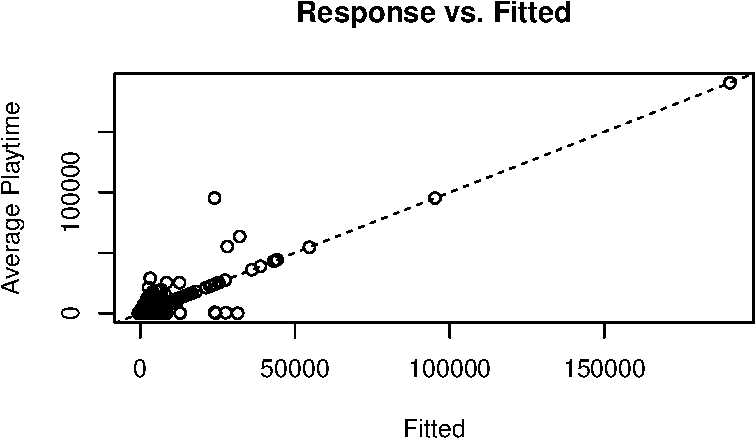
\includegraphics{proposal_files/figure-pdf/unnamed-chunk-6-1.pdf}

\hypertarget{create-pairwise-scatterplots-for-predictors-to-look-for-multicollinearity}{%
\subsection{Create Pairwise Scatterplots for Predictors to look for
multicollinearity}\label{create-pairwise-scatterplots-for-predictors-to-look-for-multicollinearity}}

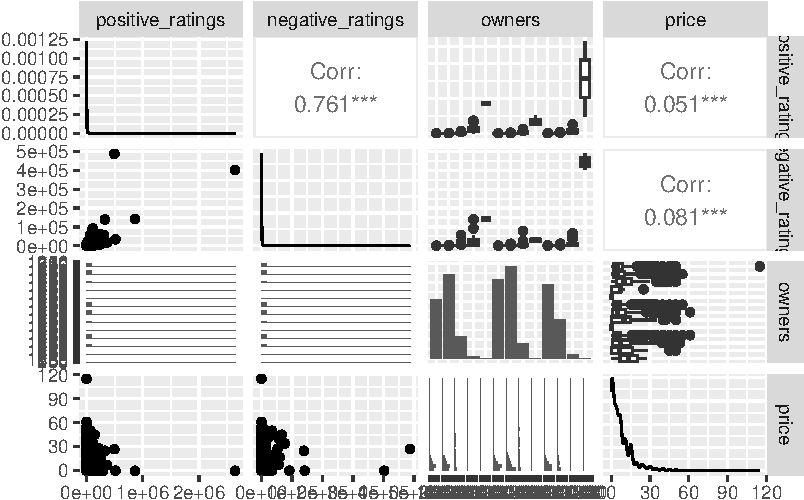
\includegraphics{proposal_files/figure-pdf/unnamed-chunk-7-1.pdf}

\hypertarget{create-residuals-vs-fitted-scatterplot-to-check-linearity-uncorrelated-errors-and-constant-variance}{%
\subsection{Create Residuals vs Fitted Scatterplot to check Linearity,
Uncorrelated Errors, and Constant
Variance}\label{create-residuals-vs-fitted-scatterplot-to-check-linearity-uncorrelated-errors-and-constant-variance}}

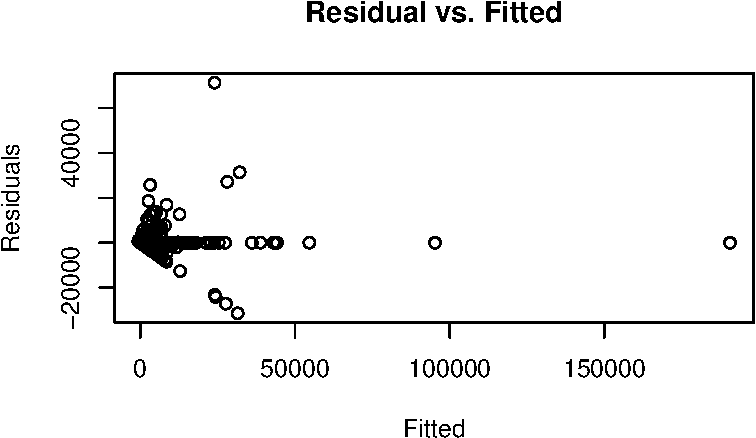
\includegraphics{proposal_files/figure-pdf/unnamed-chunk-8-1.pdf}

\hypertarget{create-residuals-vs-each-quantitative-predictor-scatterplot-to-check-linearity-uncorrelated-errors-and-constant-variance}{%
\subsection{Create Residuals vs each Quantitative Predictor scatterplot
to check Linearity, Uncorrelated Errors, and Constant
Variance}\label{create-residuals-vs-each-quantitative-predictor-scatterplot-to-check-linearity-uncorrelated-errors-and-constant-variance}}

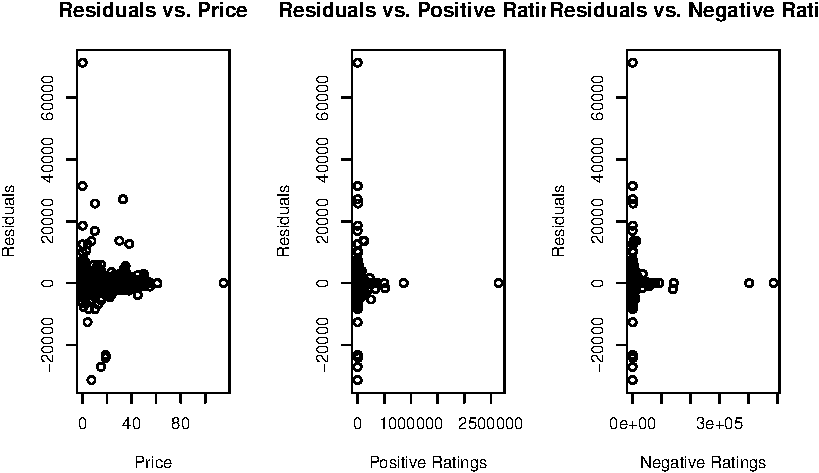
\includegraphics{proposal_files/figure-pdf/unnamed-chunk-9-1.pdf}

\hypertarget{create-boxplot-to-check-assumptions-for-categorical-predictors}{%
\subsection{Create BoxPlot to check assumptions for Categorical
Predictors}\label{create-boxplot-to-check-assumptions-for-categorical-predictors}}

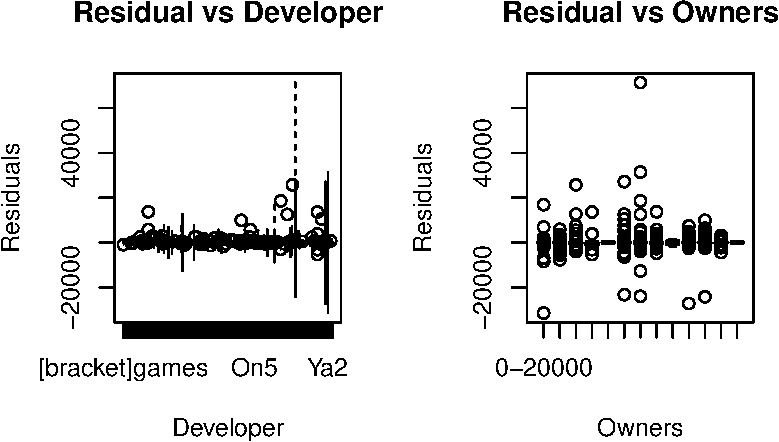
\includegraphics{proposal_files/figure-pdf/unnamed-chunk-10-1.pdf}

\hypertarget{create-normal-qq-plot-to-check-normality-assumption}{%
\subsection{Create Normal QQ Plot to check Normality
assumption}\label{create-normal-qq-plot-to-check-normality-assumption}}

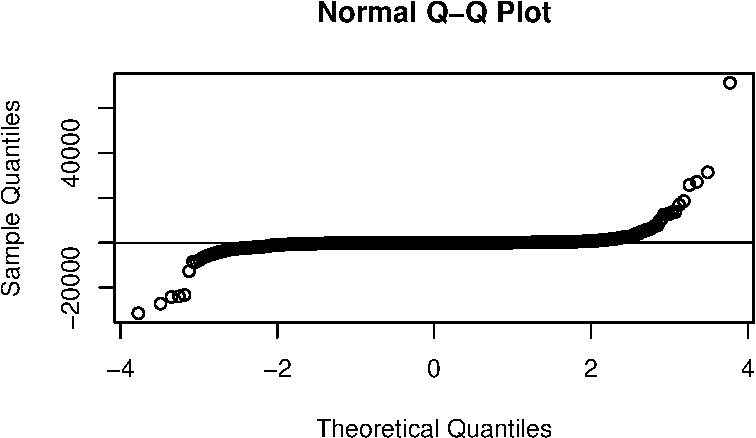
\includegraphics{proposal_files/figure-pdf/unnamed-chunk-11-1.pdf}

\newpage

\hypertarget{references}{%
\section*{References}\label{references}}
\addcontentsline{toc}{section}{References}

\hypertarget{refs}{}
\begin{CSLReferences}{1}{0}
\leavevmode\vadjust pre{\hypertarget{ref-paper1}{}}%
Brodschneider, Vinzenz, and Johanna Pirker. 2023. {``On the Influence of
Reviews on Play Activity on Steam - a Statistical Approach.''}
\emph{ResearchGate}.
\url{https://www.researchgate.net/publication/376227235_On_the_Influence_of_Reviews_on_Play_Activity_on_Steam_-_A_Statistical_Approach}.

\leavevmode\vadjust pre{\hypertarget{ref-davis2023steam}{}}%
Davis, Nik. 2023. {``Steam Store Games (Clean Dataset).''}
\url{https://www.kaggle.com/datasets/nikdavis/steam-store-games/data}.

\leavevmode\vadjust pre{\hypertarget{ref-lubridate}{}}%
Grolemund, Garrett, and Hadley Wickham. 2011. {``Dates and Times Made
Easy with {lubridate}.''} \emph{Journal of Statistical Software} 40 (3):
1--25. \url{https://www.jstatsoft.org/v40/i03/}.

\leavevmode\vadjust pre{\hypertarget{ref-paper3}{}}%
Lin, Dayi, Cor-Paul Bezemer, Ahmed E. Hassan, and Ying Zou. 2019. {``An
Empirical Study of Game Reviews on the Steam Platform.''} In \emph{Empir
Software Eng}, 24.
\url{https://doi-org.myaccess.library.utoronto.ca/10.1007/s10664-018-9627-4}.

\leavevmode\vadjust pre{\hypertarget{ref-paper2}{}}%
Luisa, Andraž De, Jan Hartman, David Nabergoj, and Samo Pahor. 2021.
{``Predicting the Popularity of Games on Steam.''} \emph{ResearchGate}.
\url{https://www.researchgate.net/publication/355110719_Predicting_the_Popularity_of_Games_on_Steam}.

\leavevmode\vadjust pre{\hypertarget{ref-jsonlite}{}}%
Ooms, Jeroen. 2014. {``The Jsonlite Package: A Practical and Consistent
Mapping Between JSON Data and r Objects.''} \emph{arXiv:1403.2805
{[}Stat.CO{]}}. \url{https://arxiv.org/abs/1403.2805}.

\leavevmode\vadjust pre{\hypertarget{ref-talia}{}}%
R Core Team. 2023. \emph{R: A Language and Environment for Statistical
Computing}. Vienna, Austria: R Foundation for Statistical Computing.
\url{https://www.R-project.org/}.

\leavevmode\vadjust pre{\hypertarget{ref-httr}{}}%
Wickham, Hadley. 2023. \emph{Httr: Tools for Working with URLs and
HTTP}. \url{https://CRAN.R-project.org/package=httr}.

\leavevmode\vadjust pre{\hypertarget{ref-dplyr}{}}%
Wickham, Hadley, Romain François, Lionel Henry, Kirill Müller, and Davis
Vaughan. 2023. \emph{Dplyr: A Grammar of Data Manipulation}.
\url{https://CRAN.R-project.org/package=dplyr}.

\leavevmode\vadjust pre{\hypertarget{ref-readr}{}}%
Wickham, Hadley, Jim Hester, and Jennifer Bryan. 2024. \emph{Readr: Read
Rectangular Text Data}. \url{https://CRAN.R-project.org/package=readr}.

\end{CSLReferences}



\end{document}
